\documentclass[11pt]{article}
\usepackage{ragged2e}
\usepackage[utf8]{inputenc}
\usepackage[catalan]{babel}
\usepackage{hyperref}
\usepackage{graphicx}
\usepackage{array}

\graphicspath{ {Images/} }

\begin{document}
\begin{titlepage}

\newcommand{\HRule}{\rule{\linewidth}{0.5mm}} % Defines a new command for the horizontal lines, change thickness here

\center % Center everything on the page
 
%----------------------------------------------------------------------------------------
%	HEADING SECTIONS
%----------------------------------------------------------------------------------------

\textsc{\LARGE Universitat de Lleida}\\[1.5cm] % Name of your university/college

\includegraphics{Images/logoUDL.jpg}\\[1cm] % Include a department/university logo - this will require the graphicx package
\textsc{\Large Grau en Enginyeria Informàtica}\\[0.5cm] % Major heading such as course name
\textsc{\large Xarxes}\\[0.5cm] % Minor heading such as course title

%----------------------------------------------------------------------------------------
%	TITLE SECTION
%----------------------------------------------------------------------------------------

\HRule \\[0.4cm]
{ \huge \bfseries Pràctica 1, Programació d’aplicacions de xarxa}\\[0.4cm] % Title of your document
\HRule \\[1.5cm]
 
%----------------------------------------------------------------------------------------
%	AUTHOR SECTION
%----------------------------------------------------------------------------------------

\begin{minipage}{0.4\textwidth}
\begin{flushleft} \large
\emph{Autor:}\\
Jordi Ricard Onrubia Palacios % Your name
\end{flushleft}
\end{minipage}
~
\begin{minipage}{0.4\textwidth}
\begin{flushright} \large
\emph{Professor:} \\
Enric Guitart % Supervisor's Name
\end{flushright}
\end{minipage}\\[4cm]

%----------------------------------------------------------------------------------------
%	DATE SECTION
%----------------------------------------------------------------------------------------
{\large \today}\\[3cm] % Date, change the \today to a set date if you want to be precise
\vfill % Fill the rest of the page with whitespace
\end{titlepage}

%%%%%%%%%%%%%%%%%%%%%%%%%%%%%%%%%
%%%%%%%%%%%%ABSTRACT%%%%%%%%%%%%%
%%%%%%%%%%%%%%%%%%%%%%%%%%%%%%%%%
\newpage
\section*{Resum}
\justify
\thispagestyle{empty}
%%%%%%%%%%%%%%%%%%%%%%%%%%%%%%%%%
%%%%%%%%%%%%INDEX%%%%%%%%%%%%%%%%
%%%%%%%%%%%%%%%%%%%%%%%%%%%%%%%%%
\newpage
\thispagestyle{empty}
\tableofcontents
%%%%%%%%%%%%%%%%%%%%%%%%%%%%%%%%%
%%%%%%%%%%%%COS%%%%%%%%%%%%%%%%%%
%%%%%%%%%%%%%%%%%%%%%%%%%%%%%%%%%
\newpage
\clearpage
\pagenumbering{arabic}
\section{Protocol UDP}
Some text
\begin{figure}[h]
    \centering
    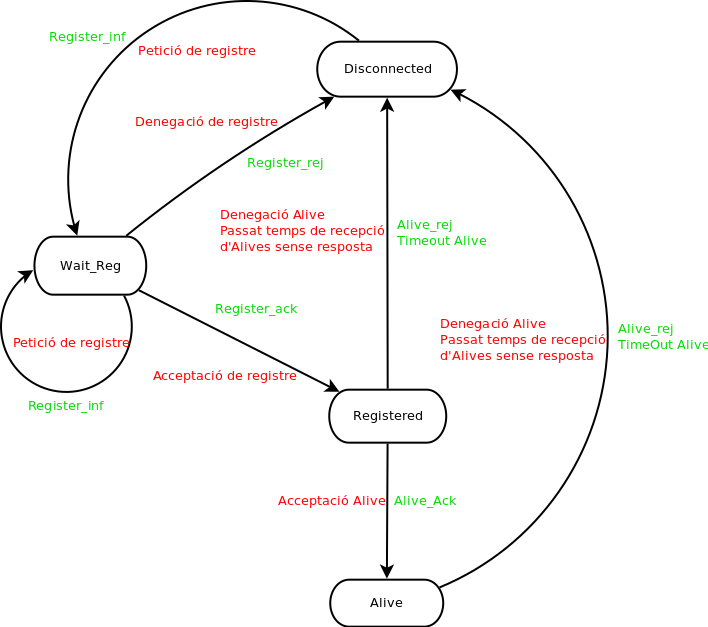
\includegraphics[width=0.8\textwidth]{UDP_diagram.png}
    \caption{Protocol UDP}
    \label{fig:ProtcolUDP}
\end{figure}

\section{Protocol TCP}
\section{Client}
\justify
Programat en: Python versió 2.7.10.
\\\\
\newpage
\begin{figure}[h]
    \centering
    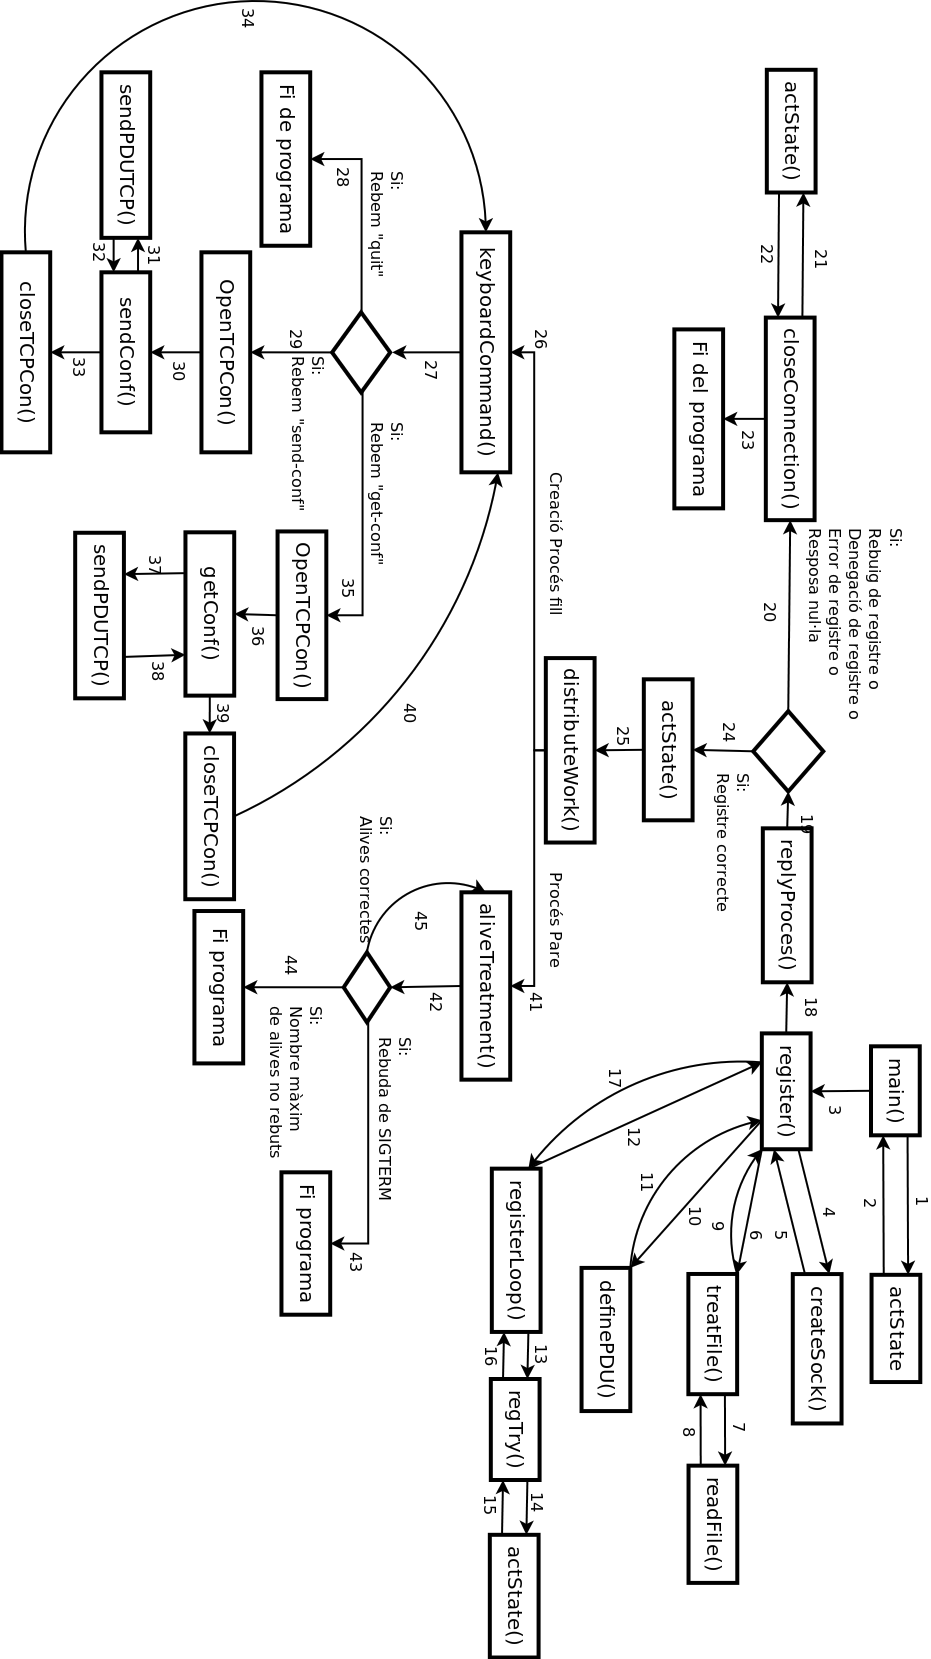
\includegraphics[width=0.8\textwidth]{Client.png}
    \caption{Client}
    \label{fig:Client}
\end{figure}
\newpage
\section{Servidor}
Compilat en: Linux versió 4.2.0 gcc versió 5.2.1.\\
Comanda utilitzada: gcc -ansi -pedantic -Wall.
%%%%%%%%%%%%%%%%%%%%%%%%%%%%%%%%%
%%%%%%%%%%%%ANEXE%%%%%%%%%%%%%%%%
%%%%%%%%%%%%%%%%%%%%%%%%%%%%%%%%%
\newpage
\section{Anexe}
	\subsection{Problemes i solucions trobats en el desenvolupament}
		\subsubsection*{Client}
\begin{enumerate}
\item Bloqueig del programa per part del recvfrom, recvfrom és una funció què s'encarrega de rebre el missatge rebut pel socket, la solució aplicada va ser posar el timeout a 0 fent-la així no bloquejant.
\item Senyal SIGTERM ignorada, la solució aplicada va ser enviarl-la continuament amb un bucle infinit.
\item Llançament de excepcions per part de Python a l'hora de detectar per teclar un ctrl-c, ls solució aplicada va ser tractar la lectura del teclat amb un try except ignorant les interrupcions de teclat.
\end{enumerate}
		\subsection*{Servidor}
\begin{enumerate}
\item Problema d'accedir i actualitzar les dades dels clients des d'altres processos. La solució ha estat fer un mmap utilitzant la llibreria sys/man.h.
\item Si els dos primers ''ALIVES'' la temporització no arriba a agafar el tercer ''ALIVE'' en cas de què fos enviat, ja que aquest arriba just en el moment en què el servidor a desconnectat al client. La solució ha estat aplicar un temporitzador per tal de què el servidor només comprovi els estats dels clients cada segon en lloc de continuament, a més a més, es permet que el temps en què haguera d'arribar ''l'ALIVE'' sigui més gran que l'especificat, exactament 1 segon més.
\end{enumerate}
\newpage
\section{Referències}
Importar constants d'un altre fitxer en Python 2.\\
\url{http://zetcode.com/lang/python/packages/}\\
Structs en Python 2.\\
\url{https://docs.python.org/2/library/struct.html}\\
UDP sockets en Python 2.\\
\url{https://wiki.python.org/moin/UdpCommunication}\\
Funcions de la llibreria Time de Python 2.\\	
\url{https://docs.python.org/2/library/time.html}\\
TCP sockets en Python 2.\\
\url{https://wiki.python.org/moin/TcpCommunication}\\
Signals en Python 2.\\	
\url{https://docs.python.org/2/library/signal.html}\\
UDP sockets en C.\\
\url{https://www.cs.rutgers.edu/~pxk/417/notes/sockets/udp.html}\\
Compartir memória en C.\\
\url{http://man7.org/linux/man-pages/man2/mmap.2.html}\\
Funcions de la llibreria Time de C.\\
\url{http://www.cplusplus.com/reference/ctime/}
\end{document}